\documentclass[border=10pt]{standalone}
\usepackage{tikz}
\usetikzlibrary{shapes,arrows,positioning,calc}

\begin{document}
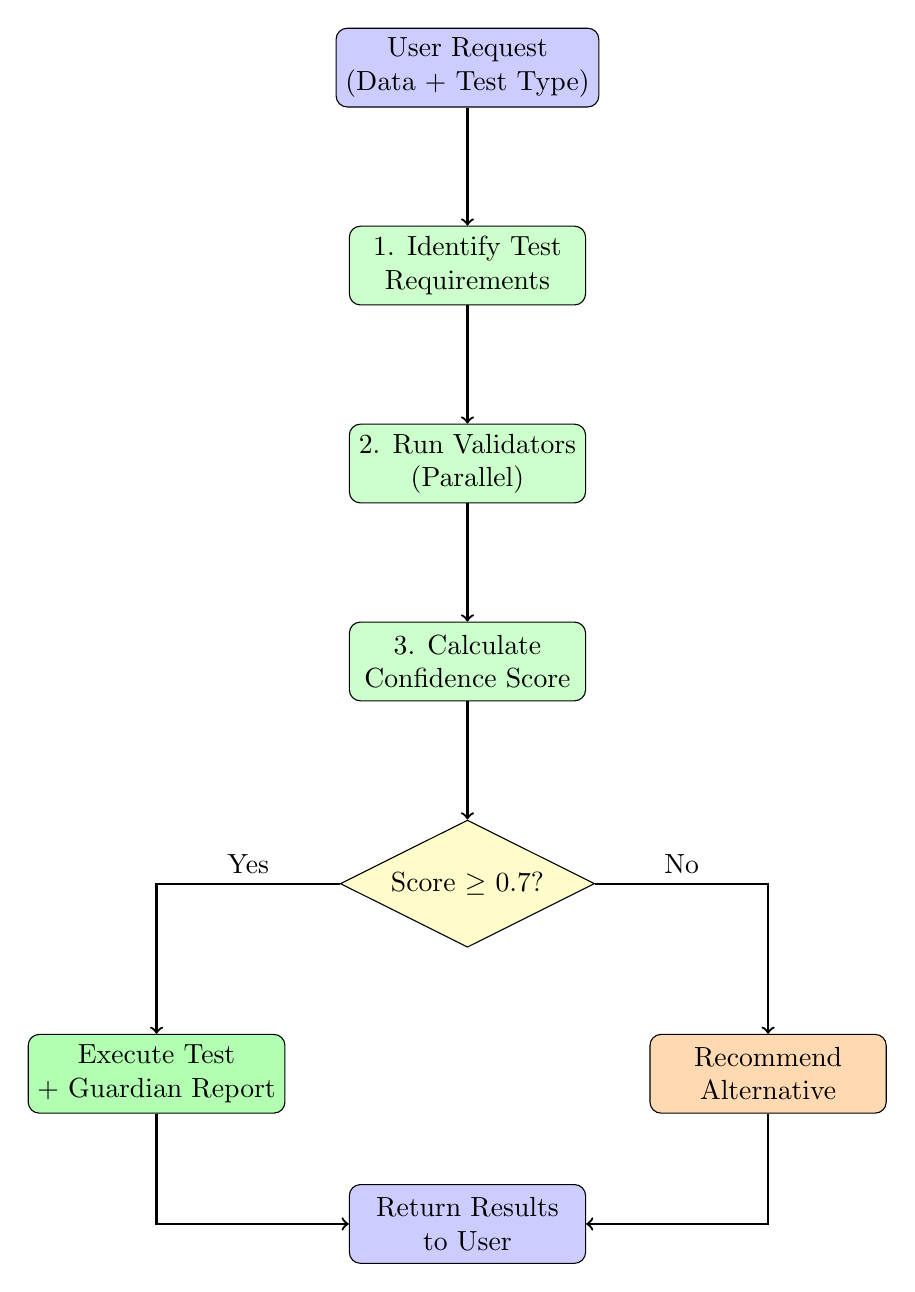
\begin{tikzpicture}[
    node distance=1.5cm,
    box/.style={draw, rounded corners, minimum width=3cm, minimum height=1cm, align=center, fill=white},
    decision/.style={draw, diamond, aspect=2, minimum width=2.5cm, align=center, fill=yellow!20},
    arrow/.style={->, thick}
]

% Start
\node[box, fill=blue!20] (start) {User Request\\(Data + Test Type)};

% Step 1
\node[box, fill=green!20, below=of start] (identify) {1. Identify Test\\Requirements};

% Step 2
\node[box, fill=green!20, below=of identify] (validate) {2. Run Validators\\(Parallel)};

% Step 3
\node[box, fill=green!20, below=of validate] (score) {3. Calculate\\Confidence Score};

% Decision
\node[decision, below=of score] (decision) {Score $\geq$ 0.7?};

% Branches
\node[box, fill=green!30, below left=1.5cm and 1.5cm of decision] (proceed) {Execute Test\\+ Guardian Report};
\node[box, fill=orange!30, below right=1.5cm and 1.5cm of decision] (recommend) {Recommend\\Alternative};

% End
\node[box, fill=blue!20, below=3cm of decision] (response) {Return Results\\to User};

% Arrows
\draw[arrow] (start) -- (identify);
\draw[arrow] (identify) -- (validate);
\draw[arrow] (validate) -- (score);
\draw[arrow] (score) -- (decision);
\draw[arrow] (decision) -| node[near start, above] {Yes} (proceed);
\draw[arrow] (decision) -| node[near start, above] {No} (recommend);
\draw[arrow] (proceed) |- (response);
\draw[arrow] (recommend) |- (response);

\end{tikzpicture}
\end{document}
